\documentclass[12pt,a4paper]{article}
\usepackage[utf8]{inputenc}
\usepackage{amsmath}
%\usepackage[brazilian]{babel}
\usepackage{breqn}
\usepackage{amsfonts}
\usepackage{amssymb}
\usepackage{graphicx}
\usepackage[margin=0.8in]{geometry}


\begin{document}
\title{\vspace{70mm}\Huge Experimento 03 - Cordas Vibrantes e Ondas Estacionárias}
\author{ Giovani Garuffi\qquad\hfill
		\textit {RA: 155559}\protect\\
		João Baraldi\hfill
		\textit{RA: 158044}\protect\\
		Lauro Cruz\hfill
		\textit{RA: 156175}\protect\\
		Lucas Schanner\hfill
		\textit{RA: 156412}\protect\\
		Pedro Stringhini\hfill
		\textit {RA: 156983}								
		}
\maketitle
\newpage
\section{Resumo}

\section{Objetivos}
Este experimento teve como objetivo principal o estudo de ondas estacionárias formadas ao longo de um fio, a fim de calcular-se o valor da densidade linear, $\mu$, desse fio.

\section{Procedimento Experimental e Coleta de Dados}

\subsection{Materiais utilizados}
Na realização deste experimento foram utilizados os seguintes materiais:
\begin{itemize}
	\item Cigarra de Frequência de 120 Hz;
	\item Trena;
	\item Fio de Nylon;
	\item Copo Plástico;
	\item Pesos de Chumbo;
	\item Polia com Suporte;
	\item Balança de Precisão.
\end{itemize}

\subsection{Procedimento}
O fio de Nylon é ligado à cigarra em uma de suas extremidades, e na outra é ligado ao copo plástico, passando pela polia, como na figura 1. Então, coloca-se os pesos de chumbo no copo, de modo que, para cada realização do experimento o valor $m$ varie, para tal, pode-se utilizar combinações lineares dos pesos adiquiridos. \\\\
Com o copo preenchido e a máxima altura do chão possível, e com a cigarra ligada, varia-se a posição da cigarra até formar-se uma onda estacionária (configuração representada na figura 2), para assim anotar-se os valores da massa $m$ no copo, previamente medido com a balança, da distância $L$ da cigarra à roldana, medido com a trena, e do número $n$ de ventres formados. \\\\
Obs.: A variação do valor de $L$ não ultrapassa de $80 \; cm$, tendo em vista que essa é, aproximadamente, a altura da mesa.


\subsection{Dados Obtidos}
Os valores de $L$ que geraram os $n$ ventres da onda, para cada valor $m$ usado, pode ser encontrados na seguinte tabela:\\

\begin{table}[!htbp]
\centering
\def\arraystretch{1.3}
\caption{Valores de $m$ usados, e os respectivos valores de $L$ para gerar $n$ ventres.}
\label{Resultados}
\begin{tabular}{|c|c|c|}
\hline
$m \; (g)$ & $L \; (cm)$ & $n$\\
\hline
$49.8 \pm 0.1$ & $130.0 \pm 0.1$ & $7$\\
$            $ & $116.8 \pm 0.1$ & $6$\\
$            $ & $ 97.3 \pm 0.1$ & $5$\\
\hline
$71.8 \pm 0.1$ & $136.5 \pm 0.1$ & $6$\\
$            $ & $115.5 \pm 0.1$ & $5$\\
$            $ & $ 90.5 \pm 0.1$ & $4$\\
\hline
$104.2 \pm 0.1$ & $134.0 \pm 0.1$ & $5$\\
$             $ & $106.5 \pm 0.1$ & $4$\\
\hline
$147.5 \pm 0.1$ & $131.0 \pm 0.1$ & $4$\\
$             $ & $ 98.5 \pm 0.1$ & $3$\\
\hline
$232.2 \pm 0.1$ & $119.3 \pm 0.1$ & $3$\\
\hline
$258.6 \pm 0.1$ & $125.5 \pm 0.1$ & $3$\\
$             $ & $ 87.5 \pm 0.1$ & $2$\\
\hline

\end{tabular} \\

\end{table}


\section{Análise dos Resultados e Discussões}
\subsection{Linearização}
A equação
$$ L = \dfrac{1}{2f} \sqrt{\dfrac{mg}{\mu}} n $$
Pode ser reescrita como
$$ L = (\dfrac{1}{2f} \sqrt{\dfrac{g}{\mu}}) \cdot n\sqrt{m} $$
$$ n \sqrt{m} = 2f\sqrt{\frac{\mu}{g}} \cdot L $$
Vemos então que deve existir uma uma relação linear entre $L$ e $n\sqrt{m}$ em que o coeficiente angular é $a = 2f \sqrt{\dfrac{\mu}{g}}$ e o coeficiente linear é $b = 0$, que pode ser verificada utilizando-se a tabela abaixo:

\begin{table}[!htbp]
\centering
\def\arraystretch{1.3}
\caption{Valores de $m$, $\sqrt{m}$ e $n\sqrt{m}$ relacionados aos comprimentos do fio $L$}
\label{Resultados}
\begin{tabular}{|c|c|c|c|c|}
\hline
$L$ $(m)$ & $n$ & $m$ $(Kg)$ & $\sqrt{m}$ $(\sqrt{Kg})$ & $n\sqrt{m}$ $(\sqrt{Kg})$ \\
\hline
$0.875\pm0.001$ & $2$ & $0.2586\pm0.0001$ & $0.5085\pm0.0001$ & $1.0171\pm0.0002$ \\
\hline
$0.905\pm0.001$ & $4$ & $0.0718\pm0.0001$ & $0.2680\pm0.0002$ & $1.0718\pm0.0007$ \\
\hline
$0.973\pm0.001$ & $5$ & $0.0498\pm0.0001$ & $0.2232\pm0.0002$ & $1.116\pm0.001$ \\
\hline
$0.985\pm0.001$ & $3$ & $0.1975\pm0.0001$ & $0.4444\pm0.0001$ & $1.3332\pm0.0003$ \\
\hline
$1.065\pm0.001$ & $4$ & $0.1042\pm0.0001$ & $0.3228\pm0.0002$ & $1.2912\pm0.0006$ \\
\hline
$1.155\pm0.001$ & $5$ & $0.0718\pm0.0001$ & $0.2680\pm0.0002$ & $1.3400\pm0.0009$ \\
\hline
$1.168\pm0.001$ & $6$ & $0.0498\pm0.0001$ & $0.2232\pm0.0002$ & $1.340\pm0.001$ \\
\hline
$1.193\pm0.001$ & $3$ & $0.2322\pm0.0001$ & $0.4819\pm0.0001$ & $1.4456\pm0.0003$ \\
\hline
$1.255\pm0.001$ & $3$ & $0.2586\pm0.0001$ & $0.5085\pm0.0001$ & $1.5256\pm0.0003$ \\
\hline
$1.300\pm0.001$ & $7$ & $0.0498\pm0.0001$ & $0.2232\pm0.0002$ & $1.562\pm0.002$ \\
\hline
$1.310\pm0.001$ & $4$ & $0.1975\pm0.0001$ & $0.4444\pm0.0001$ & $1.7776\pm0.0004$ \\
\hline
$1.340\pm0.001$ & $5$ & $0.1042\pm0.0001$ & $0.3228\pm0.0002$ & $1.6140\pm0.0008$ \\
\hline
$1.365\pm0.001$ & $6$ & $0.0718\pm0.0001$ & $0.2680\pm0.0002$ & $1.608\pm0.001$ \\
\hline

\end{tabular} \\

\end{table}

\subsection{Regressão linear}
Fazendo-se a regressão linear $n\sqrt{m}$ por $L$ obtem-se os coeficientes:
$$a = 1.3985 \pm 0.0007 \dfrac{\sqrt{Kg}}{m}$$
$$b = -0.196 \pm 0.001 \sqrt{Kg}$$
Sendo $a$ o coeficiente angular e $b$ o coeficiente linear.
Nota-se que segundo a linearização da equação original, o coeficiente linear deveria ser nulo, o que não condiz com a regressão linear dos dados experimentais. Isso se deve a erros aleatórios e erros durante as medições.
A sobreposição da reta obtida sobre os pontos da tabela pode ser vista no gráfico abaixo:

\begin{figure} [!htbp]

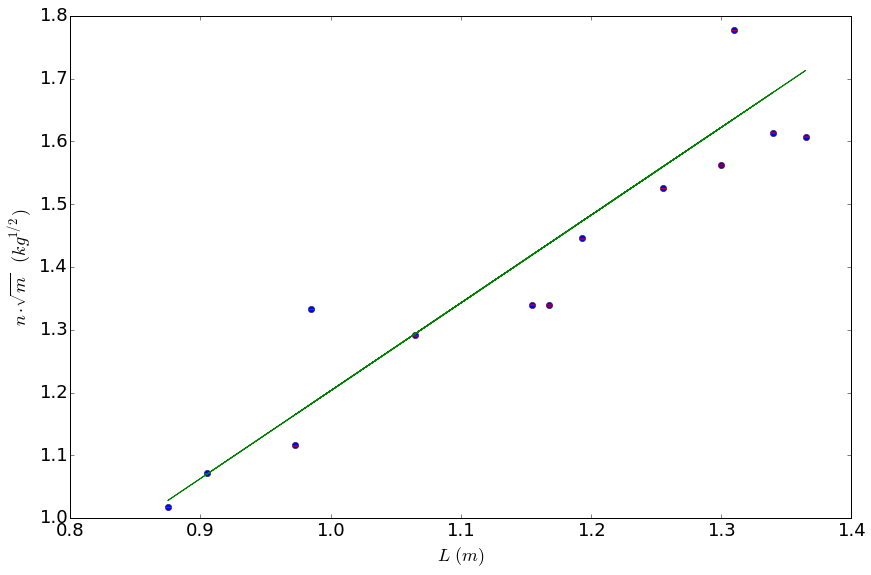
\includegraphics[scale=0.6]{graf1.png}
\caption{Gráfico da regressão linear de $n\sqrt{m}$ por $L$, sobreposta aos pontos obtidos experimentalmente.}

\end{figure}
\subsection{Densidade linear do fio}
A densidade linear do fio é a relação entre o comprimento ($L$) do fio e sua massa ($M_f$), representado por $\mu = \dfrac{M_f}{L}$.\\\\
A representação física do coeficiente linear ($a$) é:
$$a = 2f \sqrt{\dfrac{\mu}{g}}$$
Isolando $\mu$ obtemos:
$$ \mu = \dfrac{ga^2}{4f^2} $$
Considerando o valor da aceleração da gravidade 
$$g = 9.8 \; m/s^2 $$
Podemos calcular o valor da densidade linear como:
$$ \mu = 3.327 \cdot 10^{-4} \; Kg/m$$
O erro de $\mu$ é dado por:
$$ \Delta \mu = \dfrac{ga}{2f^2} \cdot \Delta a$$
E fazendo-se as devidas substituições chega-se ao valor de:
$$\Delta \mu = 3 \cdot 10^{-7} \; Kg/m$$

Assim, o valor encontrado experimentalmente não está de acordo com o valor conhecido da densidade linear do fio, de $2.340 \cdot 10^{-4} Kg/m$.

% Migués %

\section{Conclusões}


\begin{thebibliography}{9}


\end{thebibliography}

\end{document}

